\section{評価}
\label{section:評価}
\subsection{Service Workerのパフォーマンス}
\label{subsubsection:Service Workerのパフォーマンス}
Lighthouseとネットワークスロットリングを使用して、それぞれの都道府県の観光地図を読み込んだ際のパフォーマンスを計測した。キャッシュ戦略ごとのパフォーマンス指標の値の平均を図~\ref{figure:Service Workerを使用しなかった場合のパフォーマンス}、~\ref{figure:全てのネットワークレスポンスをキャッシュした場合のパフォーマンス}、~\ref{figure:画像をキャッシュした場合のパフォーマンス}、~\ref{figure:Same-Originのネットワークレスポンスをキャッシュした場合のパフォーマンス}に示す。
\begin{figure}
  \centering
  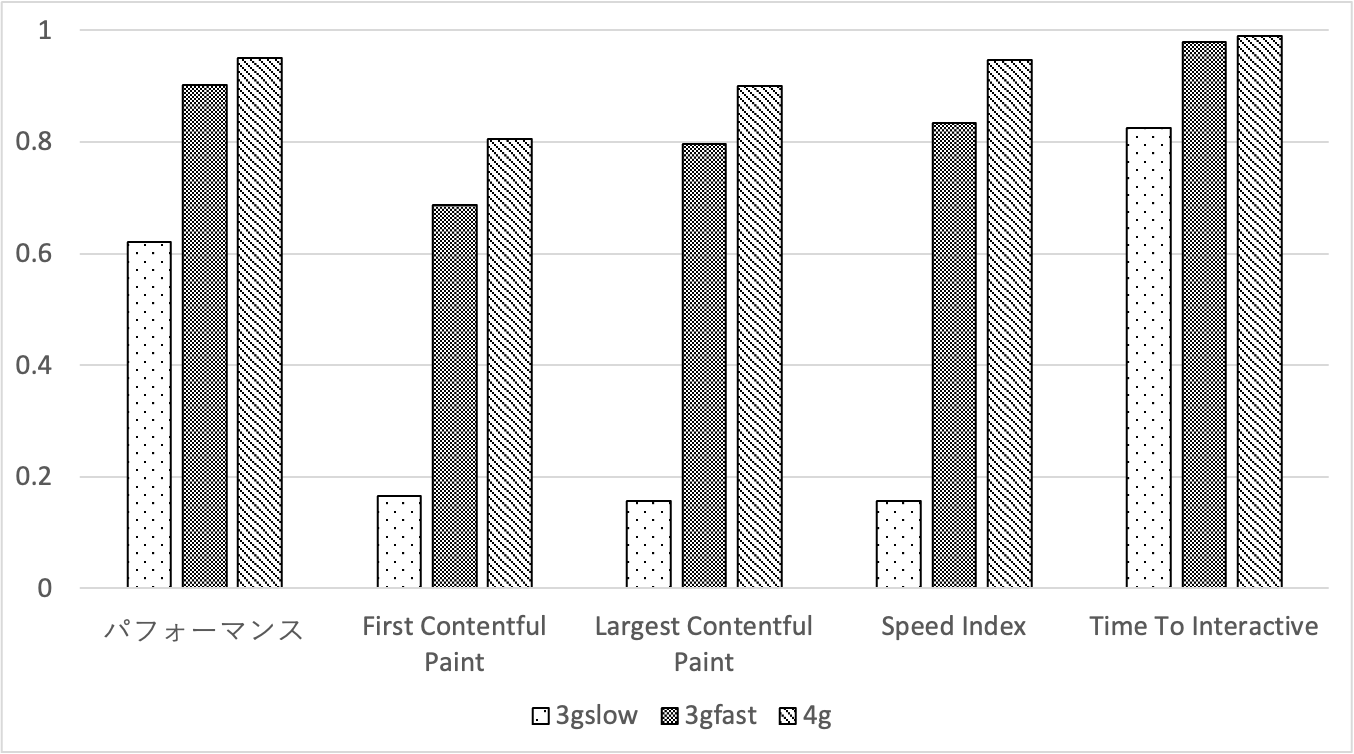
\includegraphics[width=0.9\textwidth]{images/without_service_worker.png}
  \caption{Service Workerを使用しなかった場合のパフォーマンス}\label{figure:Service Workerを使用しなかった場合のパフォーマンス}
\end{figure}
\begin{table}
  \caption{全てのネットワークレスポンスをキャッシュした場合のパフォーマンス}
  \label{table:全てのネットワークレスポンスをキャッシュした場合のパフォーマンス}
  \centering
  \begin{tabular}{|p{15em}|p{5em}|p{5em}|p{5em}|}
    \hline
    & 3gslow & 3gfast & 4g \\ \hline
    パフォーマンス & 1 & 1 & 1 \\ \hline
    First Contentful Paint & 1 & 1 & 1 \\ \hline
    Largest Contentful Paint & 1 & 1 & 1 \\ \hline
    Speed Index & 1 & 1 & 1 \\ \hline
    Total Blocking Time & 1 & 1 & 1 \\ \hline
    Cumulative Layout Shift & 1 & 1 & 1 \\ \hline
  \end{tabular}
\end{table}
\begin{figure}
  \centering
  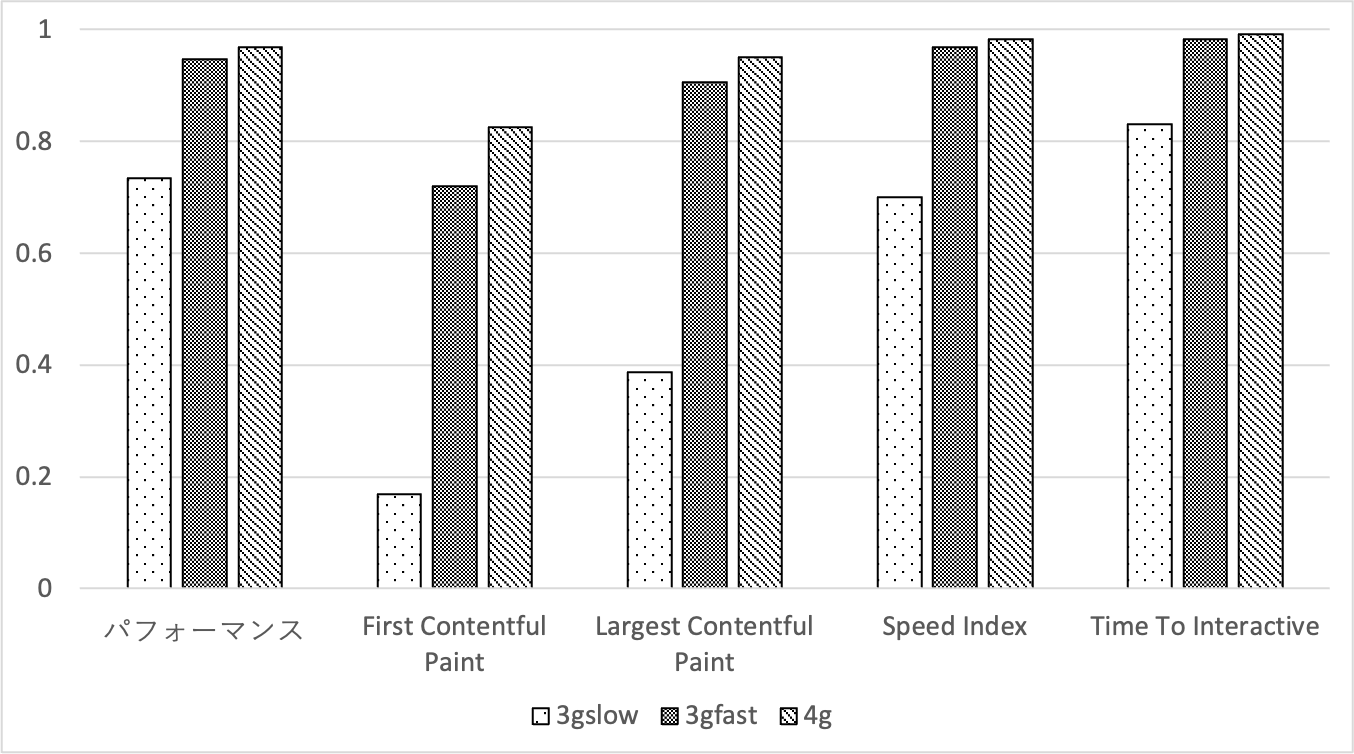
\includegraphics[width=0.9\textwidth]{images/service_worker_cache_images.png}
  \caption{画像をキャッシュした場合のパフォーマンス}\label{figure:画像をキャッシュした場合のパフォーマンス}
\end{figure}
\begin{figure}
  \centering
  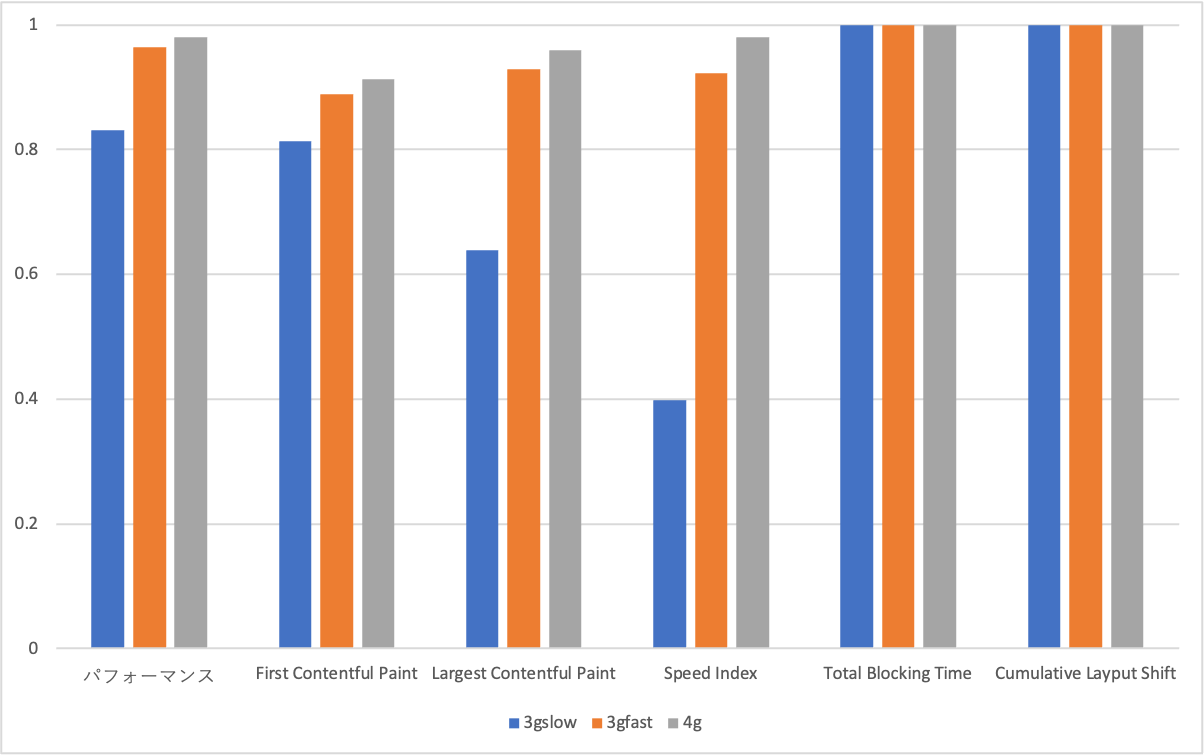
\includegraphics[width=0.9\textwidth]{images/service_worker_cache_same_origin.png}
  \caption{Same-Originのネットワークレスポンスをキャッシュした場合のパフォーマンス}\label{figure:Same-Originのネットワークレスポンスをキャッシュした場合のパフォーマンス}
\end{figure}
いずれの場合もTBTとCLSは1である。4g、3gfast、3gslowの順でパフォーマンス指標の値が大きい傾向にある。全てのネットワークレスポンスをキャッシュした場合は3gslow、3gfast、4gのいずれの場合も全ての指標の値は1である。画像をキャッシュした場合はFCPが最も通信速度の低下の影響を受けやすく、SIが最もその影響を受けにくいことが分かる。逆に、Same-Originのネットワークレスポンスのキャッシュした場合はSIが最も通信速度の低下の影響を受けやすく、SCPが最もその影響を受けにくいことが示されている。

3gfastに比べてアップリンクがおよそ12倍、ダウンリンクがおよそ6倍である4gプロファイルを使用した場合であってもほとんどのパフォーマンス指標の値は1未満である。全体的に見ると、3gslowと3gfast間のパフォーマンス指標の値の増加率は3gfastと4g間の増加率よりも大きい。